\documentclass[prd,onecolumn,amsmath,amssymb,floatfix,superscriptaddress,notitlepage]{revtex4-1}
\usepackage{graphicx,epsfig}
\usepackage{caption}
\def\be{\begin{equation}}
\def\ee{\end{equation}}
\def\ben{\begin{equation*}}
\def\een{\end{equation*}}

\def\ba{\begin{eqnarray}}
\def\ea{\end{eqnarray}}
\def\ban{\begin{eqnarray*}}
\def\ean{\end{eqnarray*}}
\newcommand{\refsec}[1]{section~\ref{sec:#1}}
\newcommand{\refeq}[1]{Eq.~(\ref{eqn:#1})}
\newcommand{\refssec}[1]{section~\ref{subsec:#1}}
\newcommand{\reffig}[1]{Fig.~\ref{fig:#1}}
\newcommand{\refFig}[1]{Fig.~\ref{fig:#1}}
\newcommand{\reftab}[1]{Tab.~\ref{tab:#1}}

\newcommand{\bl}{{\bf l}}
\newcommand{\bL}{{\bf L}}


%%% BEGIN DOCUMENT
\begin{document}
\title{CMB DC Mode}
\author{}
\affiliation{Department of Astronomy \& Astrophysics, University of Chicago, Chicago IL 60637}
\date{\today}

\maketitle


\section{variance test}



\begin{figure}[htbp]
\begin{center}		
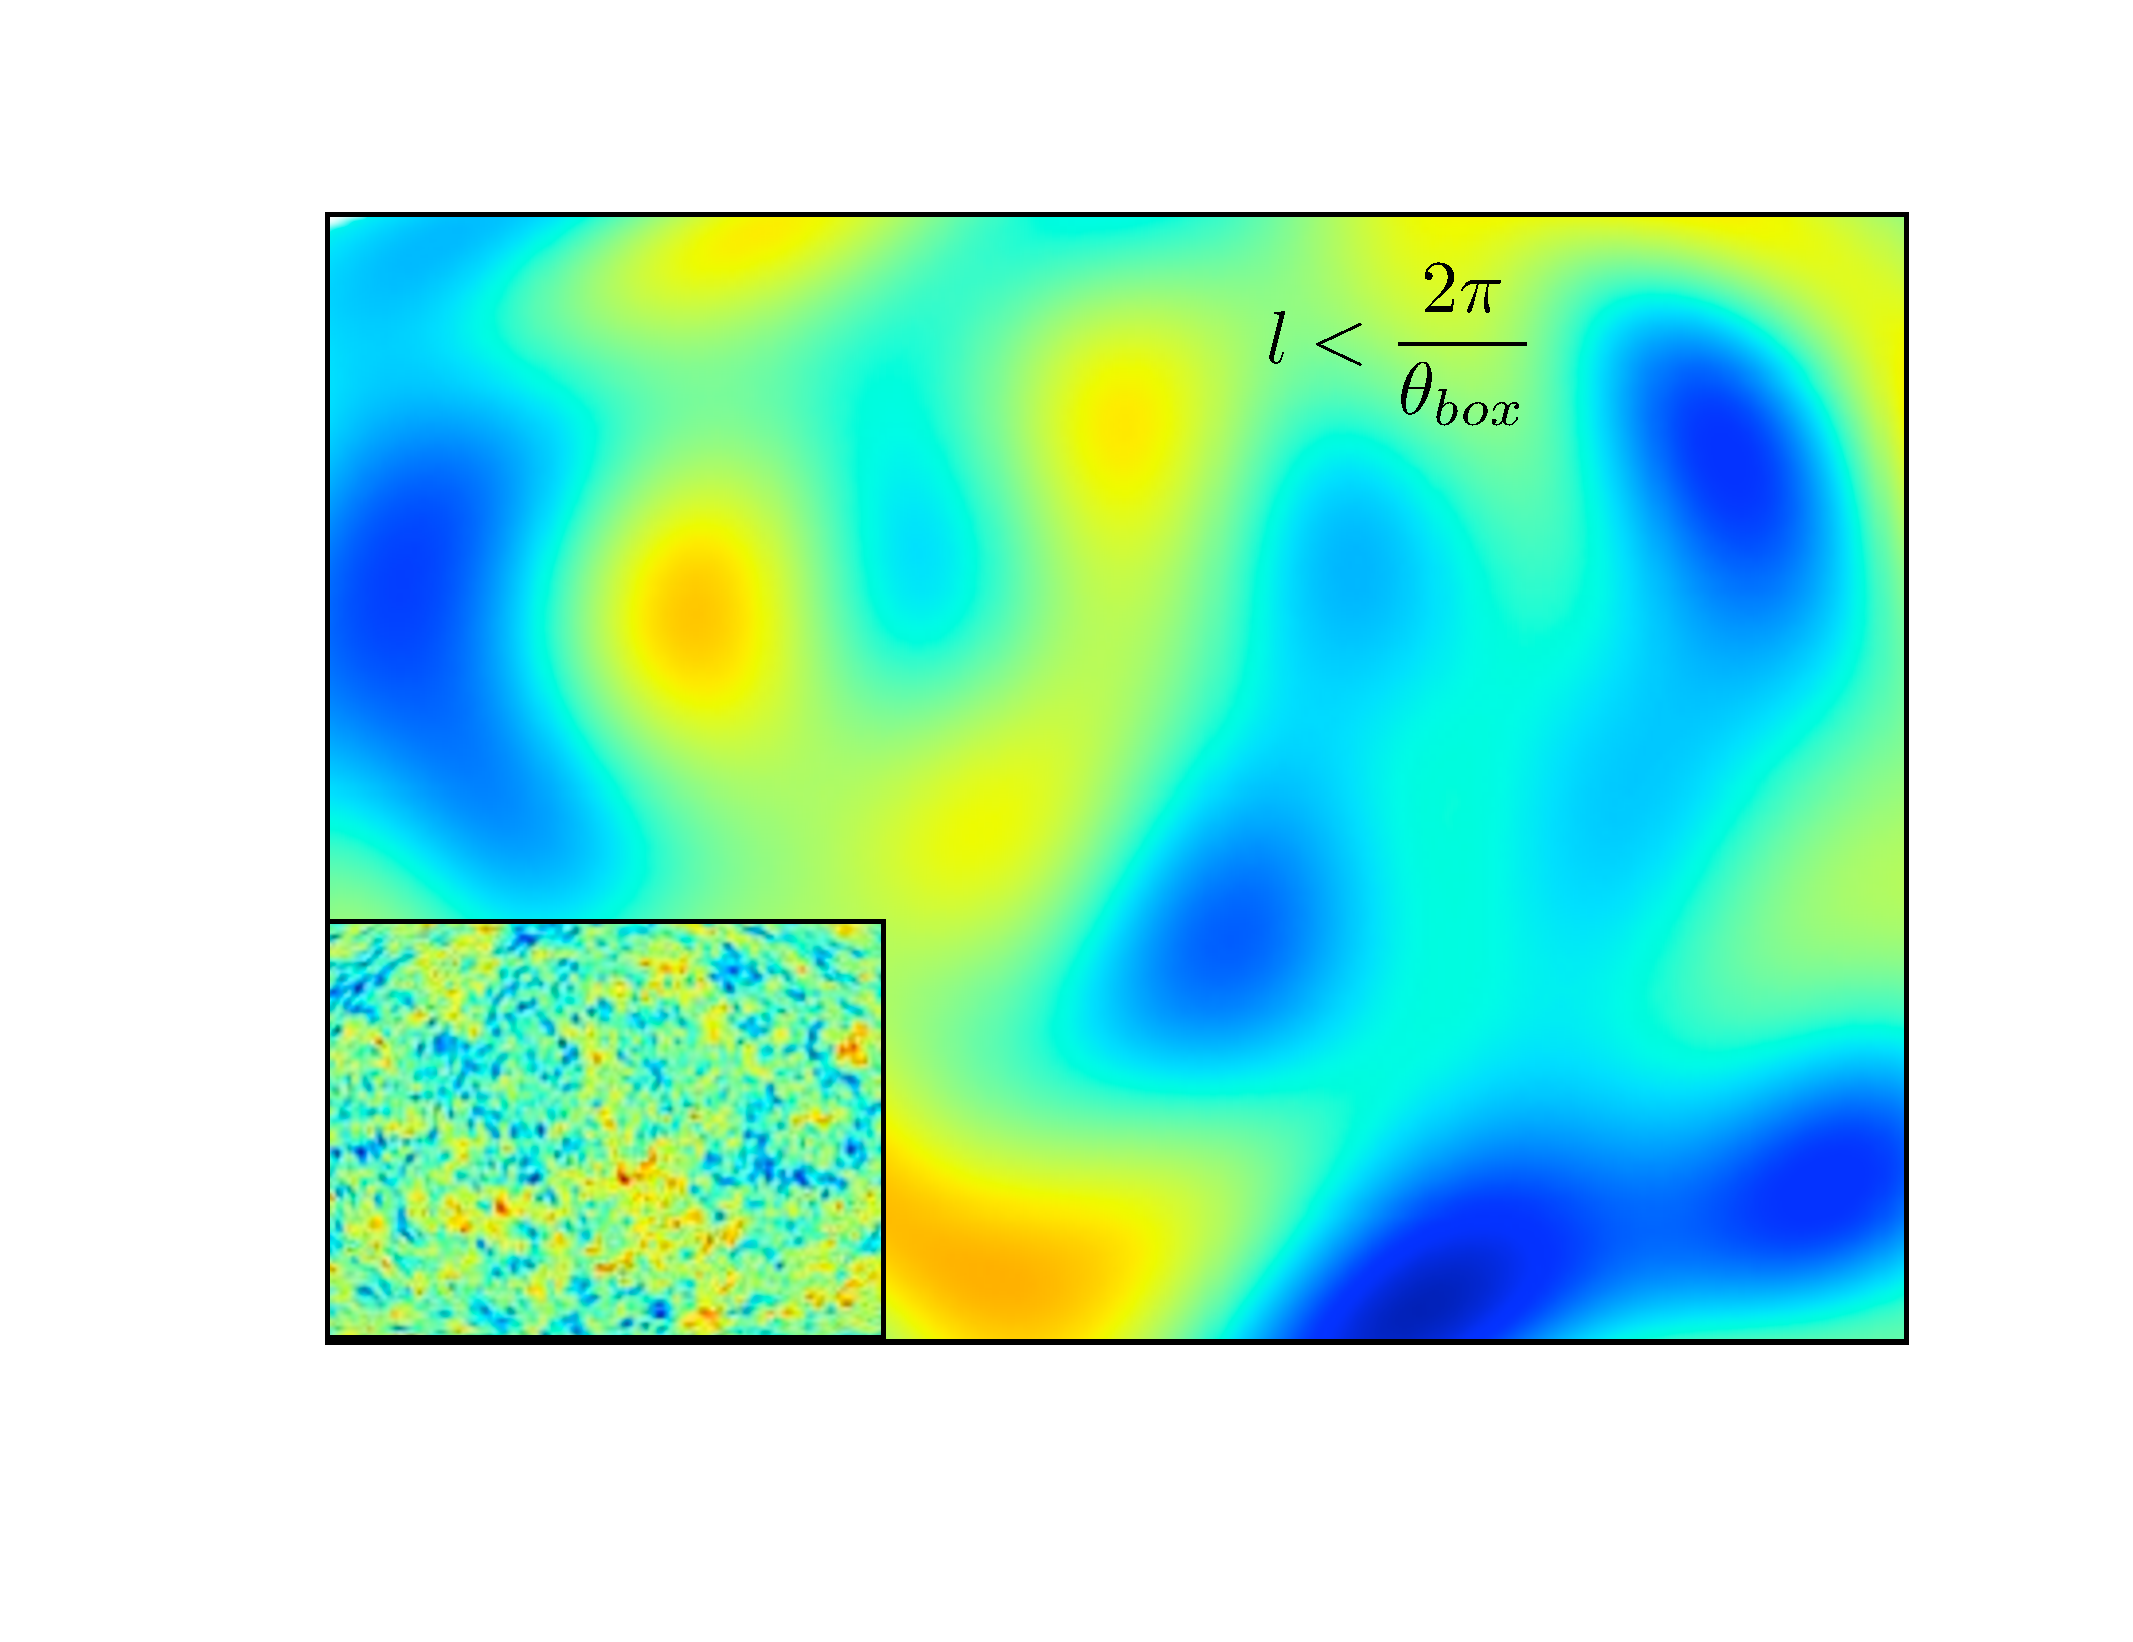
\includegraphics[scale=0.3]{./images/box.pdf}
%\label{default}
\end{center}
\end{figure}


One way to compute the variance is just to sum over all the modes that are super-sample mode considering the width of the box $\theta_{box}\rightarrow l_{max}=\frac{2\pi}{\theta_{box}}$:

\be \label{eqn:lmax}
(\sigma^{\kappa})^{2}=\sum_{0}^{l_{max}=\frac{2\pi}{\theta_{box}}}\frac{2\ell+1}{4\pi}C_{\ell}^{\kappa}
\ee




\begin{figure}[htbp]
\begin{center}
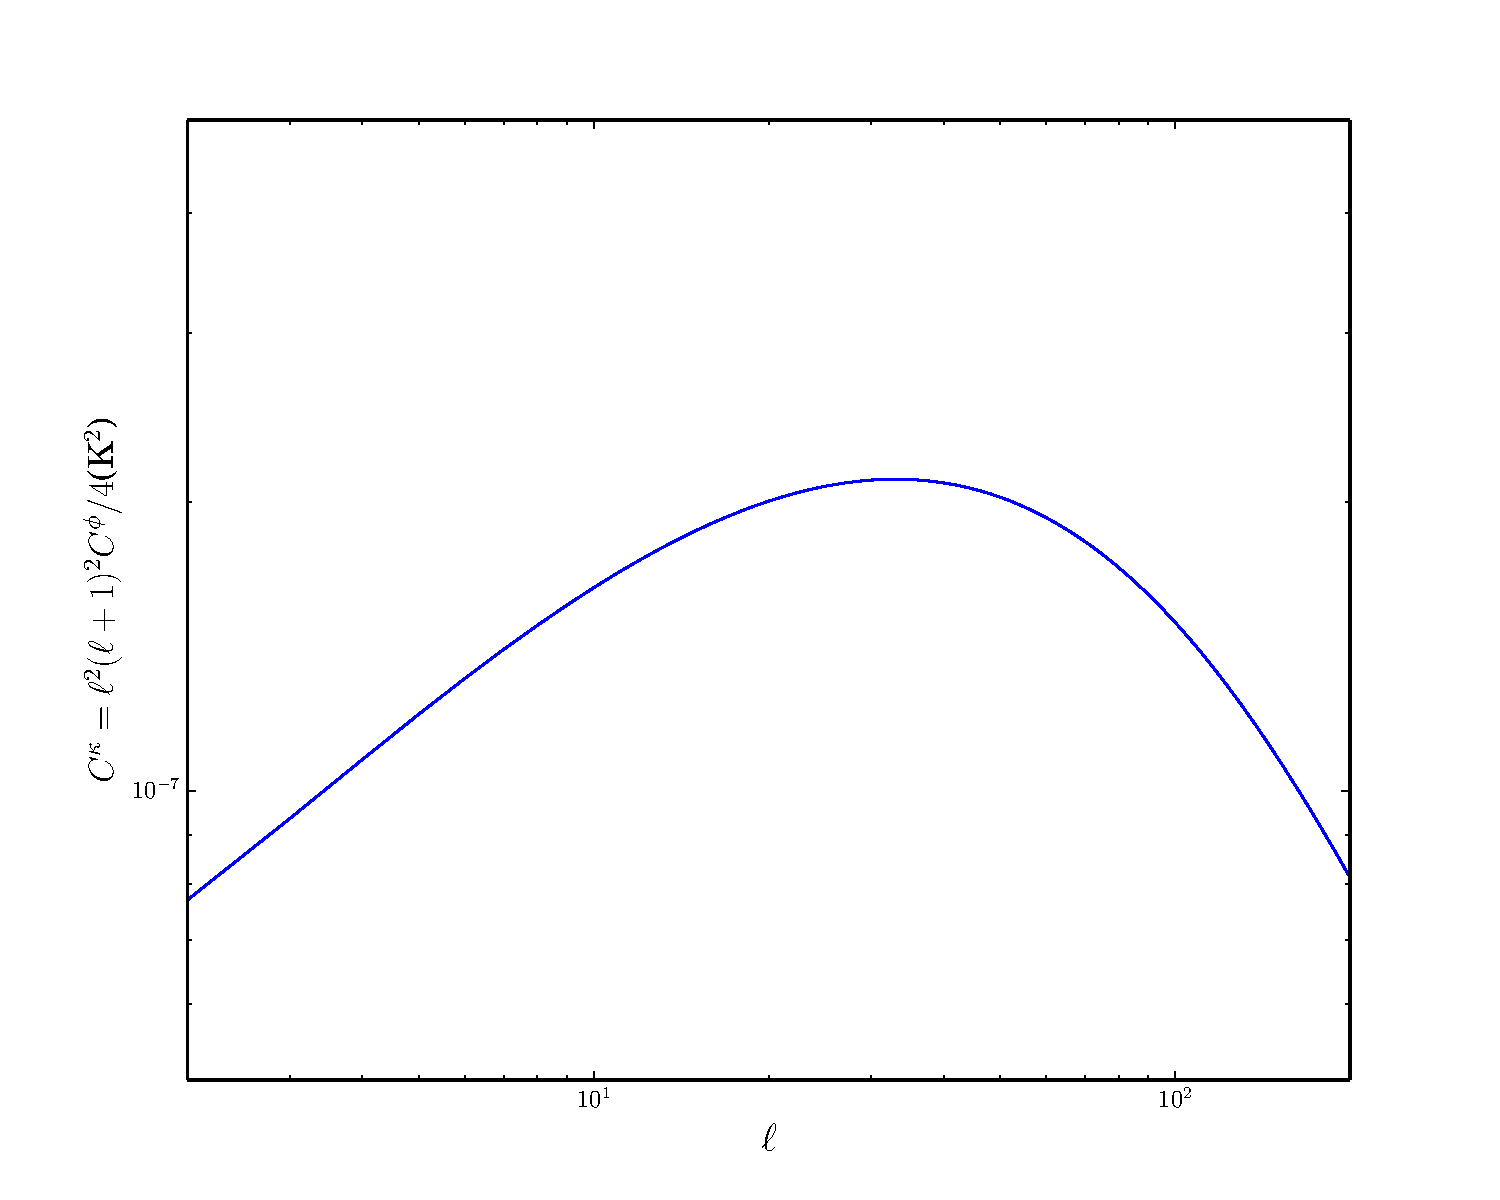
\includegraphics[scale=0.4]{./images/Ckappa.pdf}
\caption{Power spectrum}
%\caption{default}
%\label{default}
\end{center}
\end{figure}

where the convergence power is releted to the lensing one by $C^{\kappa}=\ell^{2}(\ell+1)^{2}C^{\phi}/4$.

Increasing the size of the survey, reduce the number of large scale modes that can be consider as super-survey, and so the variance is reduced. This reduce the ``super sample covariance '' effect. 
Now the width of the survey could be derived from the total area, assuming it covers a circular area, by $\pi \theta_{box}^{2}=\text{Area}(\frac{\pi}{180})^{2}$. 
In this case $l_{max}=\frac{2\pi}{\theta_{box}}=\frac{2\pi}{\sqrt{(\text{tot Area})/\pi} (\pi/180)}=\frac{360\sqrt\pi}{\sqrt{\text{tot Area}}}=\frac{638}{\sqrt{\text{tot Area}}}$, where the total area has to be expressed in degree squared. For a 1000 deg$^{2}$ we get $l_{max}\approx20$

We want to compare this effect to the precision on the measurement of the angular size of sound horizon at last scattering, cause the effect of this background mode can be seen as if the fraction of the sky tested by the survey would have been sitted on a slightly over or under dense region, a slightly closed or open universe. The effect on the power spectrum is the same as a change in the curvature: a shift in the power spectrum.
The current precision reach by planck is $\frac{\sigma_{\theta^{\star}}}{\theta^{\star}}=\frac{0.00006}{1.041}=0.00057$.

We can improve this rough estimate by introducing a simple window function for the survey.

The variance in a 2D flat sky approximation become:
\be
\sigma^{2}_{\kappa}=\int \frac{d^{2}~q}{(2\pi)^{2 }}|\tilde W(q)|^{2} P(q),
\ee
where $\tilde W(q)$ is the fourier transform of the window function (we used the usual Fourier transform conventions).
As a window we can choose a uniform circular disk or radius $R=\theta_{box}$ (normalized so that $\int d^{2}x ~W(x)=1$) in the small angle approximation.
We have
\ba
|\tilde W(q)|&=&\int d^{2}x e^{-i q\cdot x} \Theta(r-R)/(\pi R^{2})\\
&=&\int_{0}^{\infty} x~dx \int_{0}^{2\pi} d\theta e^{-i qx\cos\theta} \Theta(r-R)/(\pi R^{2})\\
&=&1/(\pi R^{2}) \int_{0}^{R} xdx~ \int_{0}^{2\pi} d\theta e^{-i qx\cos\theta} \\
&=&1/(q \pi R^{2}) \int_{0}^{R} xdx~ 2\pi q J_{0}(xq) \\
&=&\frac{2\pi}{\pi R^{2} q^{2}}\int_{0}^{R} d(xq) xq J_{0}(xq) \\
&=&\frac{2\pi}{\pi R^{2} q^{2}}Rq J_{1}(Rq) \\
&=&\frac{2~J_{1}(Rq)}{Rq}. \\
\ea
We have used two properties of bessel functions
\ba
&&J_{n}=\frac{i^{-n}}{\pi}\int_{0}^{\pi}d\theta e^{ix\cos\theta}cos(n\theta)\\
&&\frac{d}{dx}[xJ_{1}(x)]=xJ_{0}(x)\\
\ea


The variance become:
\ba \label{eqn:integral}
\sigma_{\kappa}^{2}&=&\int \frac{d^{2}~\ell}{(2\pi)^{2}} \left(\frac{2~J_{1}(\ell~\theta_{box})}{\ell~\theta_{box}}\right)^{2} C_{\ell}\\
&=&\int \frac{d\ell}{(2\pi)} \ell \left(\frac{2~J_{1}(\ell~\theta_{box})}{\ell~\theta_{box}}\right)^{2} C_{\ell}
\ea
It can also be approximated by a sum 
\be \label{eqn:approx}
\sigma_{\kappa}^{2}=\sum \frac{2\ell+1}{4\pi} \left(\frac{2~J_{1}(\ell~\theta_{box})}{\ell~\theta_{box}}\right)^{2} C_{\ell}.
\ee


\begin{figure}[htbp]
\begin{center}
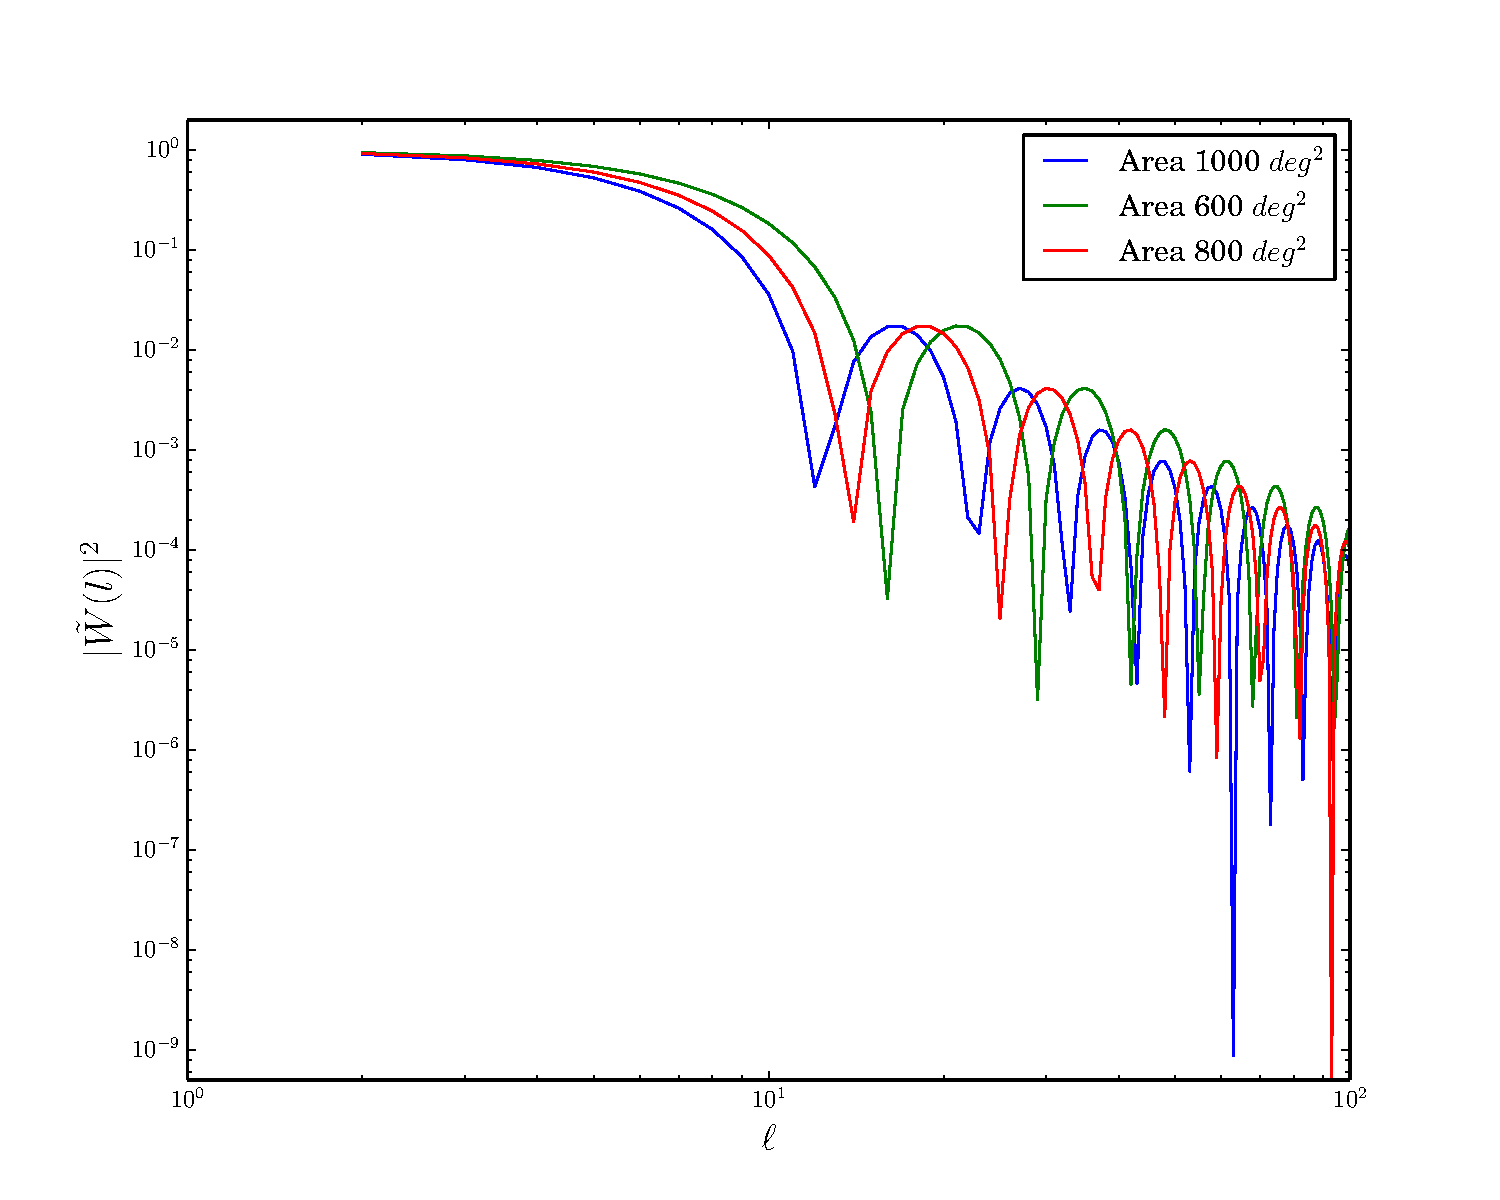
\includegraphics[scale=0.6]{./images/window.pdf}
%\caption{default}
%\label{default}
\end{center}
\end{figure}

\begin{figure}[htbp]
\begin{center}
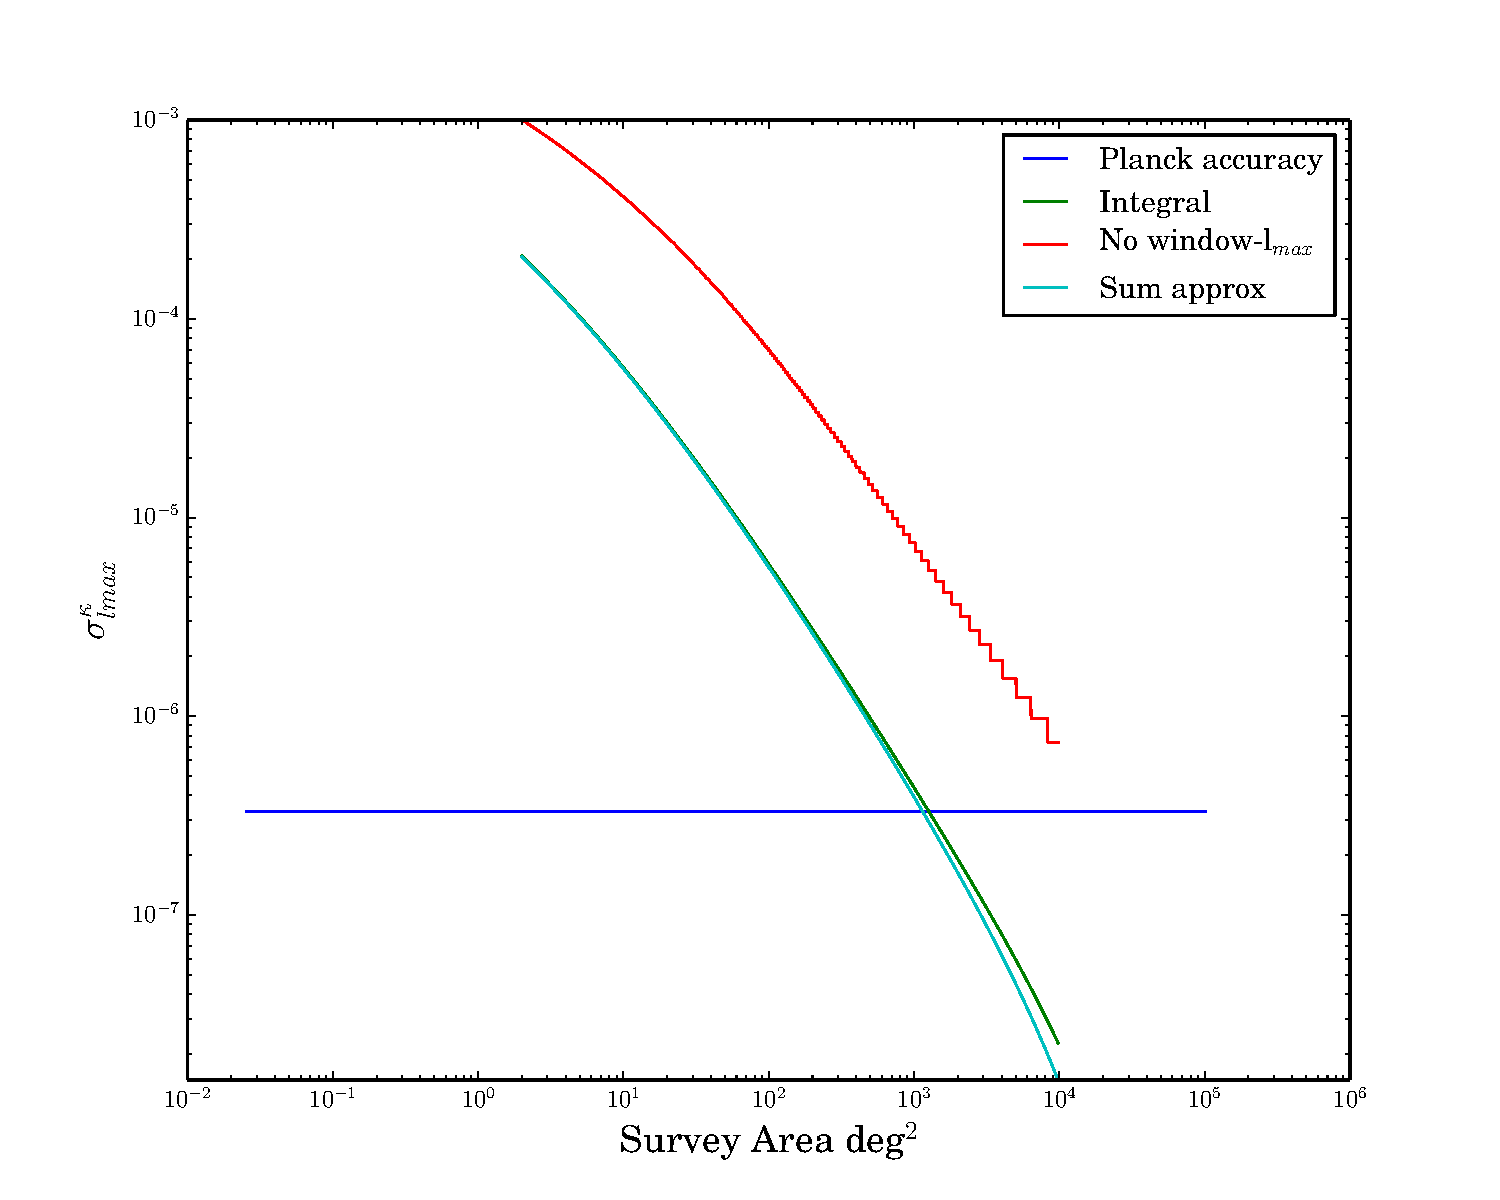
\includegraphics[scale=0.6]{./images/variance.pdf}
\caption{Integral correspond to \refeq{integral} Sum approximation is \refeq{approx} . No window lmax correspond to \refeq{lmax} which I think is pretty different cause it is like having a rectangle window function in Fourier space which give you an un-normalized sync window function in space domain. }
%\label{default}
\end{center}
\end{figure}




\section{Fisher\_estimate}

I compute the value of  $C^{\rm{fid}}_{\ell}$s using CAMB and with those I compute the Fisher estimates of the effect we are looking for, given the accuracy (beam and white noise) of a detector. See Wayne's notes.

The super sample modes shift the CMB power spectrum and so we have:
\begin{equation}\label{eqn:Cfiducial}
C_l = C_l^{\rm fid} \left[ 1+ \frac{\partial \ln (l^2 C_l^{\rm fid} )}{\partial \ln l} s \right].
\end{equation}
Notice that the effect is stronger where the derivatives are bigger, near the peaks.
Now we can perform a Fisher estimate of $\sigma_s^2$ (no other parameters marignalized) and compare it to $\sigma_\kappa^2$.  
I compute:
\begin{equation}
\frac{\partial C_{\ell}}{\partial s}=C^{\rm fid}\frac{\partial \ln (l^2 C_l^{\rm fid}) }{\partial \ln l},
\end{equation}
directly from the spline function I use to fit the spectrum (maybe we need something more accurate?); after that, following the fisher formalism:
\ben
F_{ss}=\sum_{\ell}\frac{1}{(\delta C_{\ell})^{2}}\left( C^{\rm fid}\frac{\partial \ln (l^2 C_l^{\rm fid} )}{\partial \ln l}\right)^{2}
\een
\ben
F_{ss}=\sum_{\ell}\frac{(2\ell+1)f_{\rm sky}}{2[C^{\rm{fid}}_{\ell}+N_{\ell}]^{2}}\left( C^{\rm fid}\frac{\partial \ln (l^2 C_l^{\rm fid} )}{\partial \ln l}\right)^{2}
\een
Now we can estimate the accuracy on $\sigma_{s}^{2}$ using $\sigma_{s}^{2}=F_{ss}^{-1}$

\be
N_{\ell}=\left( 4 \mu K \left(\frac{\pi}{10800}\right)\right)\exp\{-\ell(\ell+1)\theta\left(\frac{\pi}{10800}\right)/(8\log 2)\}.
\ee
I put the equation explicitly cause I am not sure that when they quote an accuracy they mean this or the same divided by the T$_{CMB}$.

The next questions is where in the ($\ell_{max},f_{sky}$) region the effect $\sigma_{\kappa}^{2}$ is bigger than the accuracy we can reach in measuring it estimated using the fisher matrix approach, $\sigma_{s}^{2}$.
This can be seen in \reffig{comparison} where we have plotted $\sigma_{s}^{2}f_{sky}$ as a function of $l_{max}$ and horizontal lines that correspond to the value of $\sigma_{\kappa}^{2}f_{sky}$ for different survey areas.


\begin{figure}[htbp]
\begin{center}
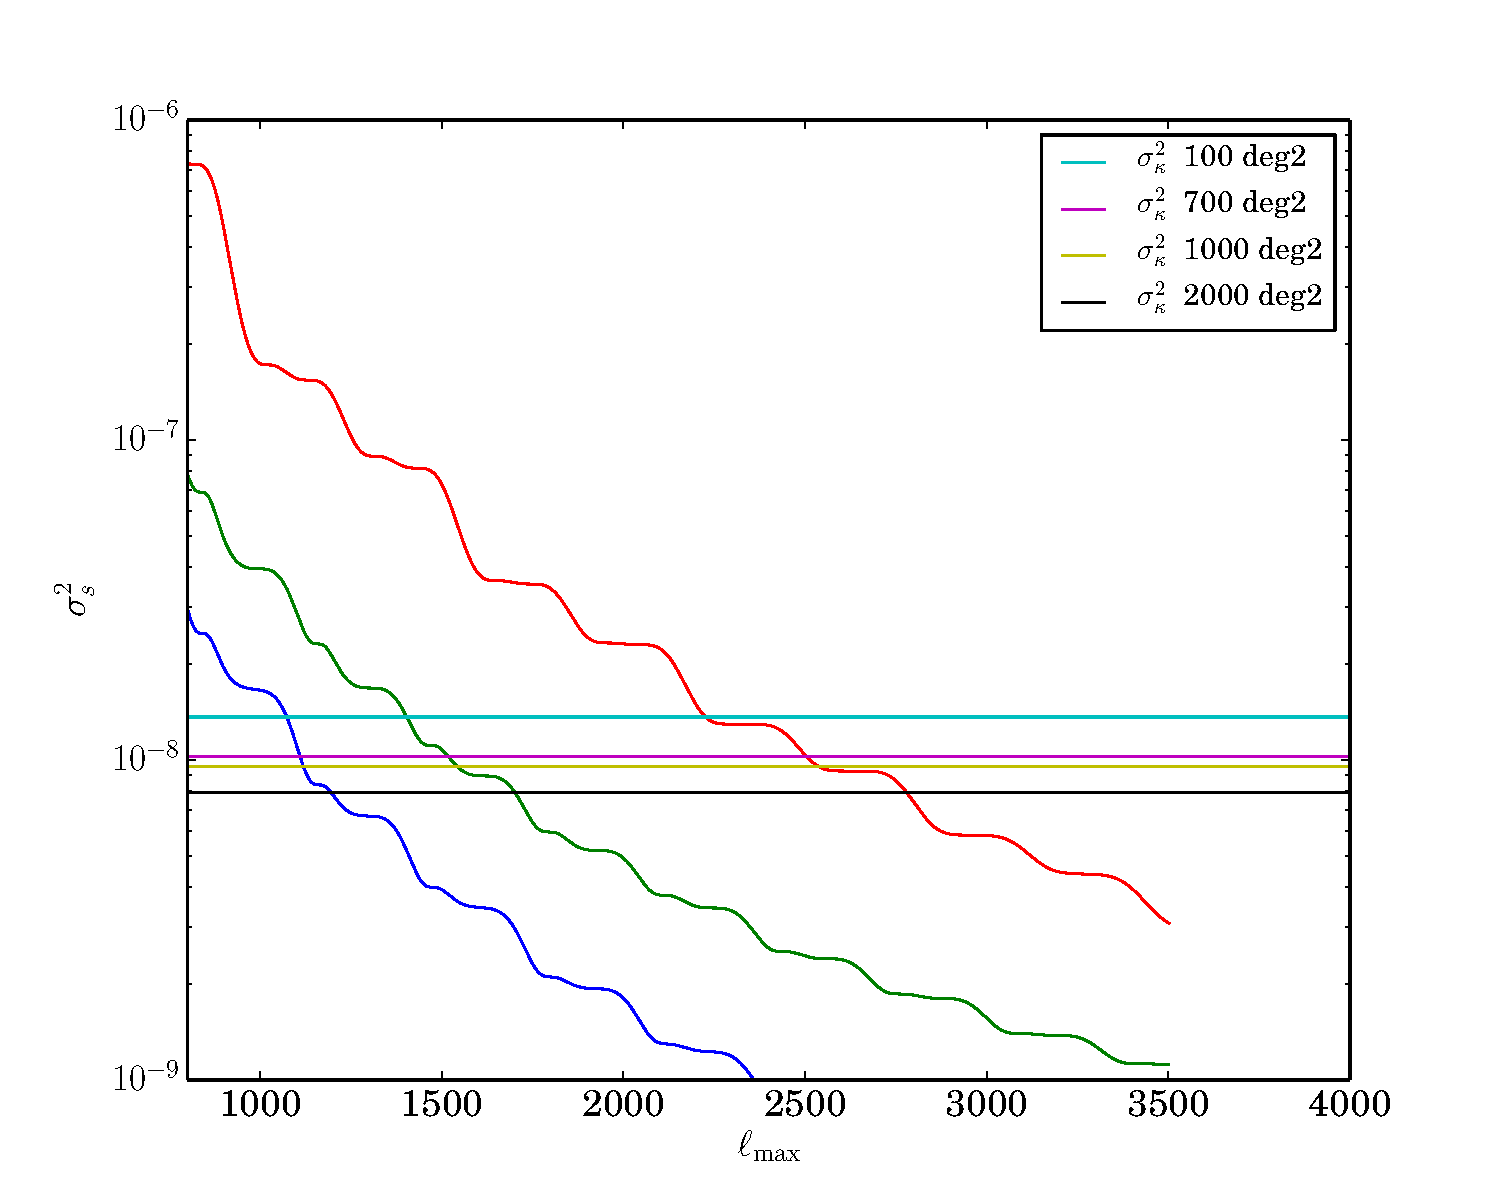
\includegraphics[scale=0.6]{./Images/variancecompare.pdf}
\caption{The solid curves represent $\sigma_{s}^{2}f_{sky}$ estimated from power spectra as a function of $l_{max}$. 
The red one is computed using the temperature data only $F_{ss} = {2 \over f_{sky}(2\ell+1)} \left(\frac{\partial \ln(\ell^{2}C^{T})}{\partial \ln\ell}\right)^{2}$;The green one is computed using the E-mode data only $F_{ss} = {2 \over f_{sky}(2\ell+1)} \left(\frac{\partial \ln(\ell^{2}C^{E})}{\partial \ln\ell}\right)^{2}$, and the blue one combine the 2 set of data using the full expression \refeq{fishertot2}.
Horizontal lines  correspond to the value of $\sigma_{\kappa}^{2}f_{sky}$ for different survey areas.}
\label{fig:comparison}
\end{center}
\end{figure}



\subsection{Polarization}

We expect the effect of the super sample covariance to be bigger in the case of the lensed polarization field, Because the unlensed polarization peaks are rather sharper than in the temperature case, this actually means that the effect of lensing is quantitatively more important on the $C_{l}^{E}$ spectrum. Let us start, in the flat sky approximation, by computing the E field trispectrum:
\be
<\tilde E(\ell_{1})~\tilde E(\ell_{2})~\tilde E(\ell_{3})~\tilde E(\ell_{4})> (2\pi)^{2} \delta(\ell_{1}+\ell_{2}+\ell_{3}+\ell_{4})\tilde T(\ell_{1}+\ell_{2}+\ell_{3}+\ell_{4})
\ee
As we did for the temperature field, we can express the lensed field respect to the unlensed one by expanding in series the spin-2 component of the polarization tensor 
\ba
\tilde P(\mathbf{n})&=&P(\mathbf{n}+\nabla \phi)\nonumber\\
&\approx& P(\mathbf{n})+\nabla \phi \nabla P(\mathbf{n})+ ...\nonumber
\ea
Using the harmonic expansion definitions in flat sky:
\ba
P=Q+iU=-\int\frac{d^{2}\mathbf{l}}{2\pi}[E(\mathbf{l})+iB(\mathbf{l})]e^{2i\phi_{l}}e^{i\mathbf{l}\mathbf{n}}
\ea
we get
\ba
\tilde E(\mathbf{l})&\approx& E(\mathbf{l})-\int\frac{d^{2}\mathbf{l'}}{2\pi}~\mathbf{l'}\cdot(\mathbf{l}-\mathbf{l'})\cos2(\phi_{l}-\phi_{l'})\psi(\mathbf{l}-\mathbf{l'})E(\mathbf{l'})\nonumber\\
&&-\frac12 \int\frac{d^{2}\mathbf{l_{1}}}{2\pi}\frac{d^{2}\mathbf{l_{2}}}{2\pi}~ \cos2(\phi_{l}-\phi_{l'}) ~\bl_{1}(\bl_{1}+\bl_{2}-\bl)~\bl_{1}\cdot\bl_{2}E(\bl_{1})\psi(\bl_{2})\psi^{*}(\bl_{1}+\bl_{2}-\bl)\\
\tilde B(\mathbf{l})&\approx&-\int\frac{d^{2}\mathbf{l'}}{2\pi}~\mathbf{l'}\cdot(\mathbf{l}-\mathbf{l'})\sin2(\phi_{l}-\phi_{l'})\psi(\mathbf{l}-\mathbf{l'})E(\mathbf{l'})
\ea
neglecting higher order in $\phi$ and primordial un-lensed B modes.

We are interested in the connected part of the lensed trispectrum $<\tilde X(\bl_{1})\tilde X(\bl_{2})\tilde X(\bl_{3})\tilde X(\bl_{4})>_{c}$ with $XXXX=\{EEEE,BBBB,EETT\}$ in a particular configuration where the modes are coupled together via a long wavelength mode \bL.

For example in the EEEE case we have

\ba
<\tilde E(\bl_{1})\tilde E(\bl_{2})\tilde E(\bl_{3})\tilde E(\bl_{4})>_{c}&\approx& \frac{1}{2(2\pi)^{2}}\delta(\bl_{1}+\bl_{2}+\bl_{3}+\bl_{4})\\
&& \times \left[ C^{\psi}_{|\bl_{1}+\bl_{3}|}C^{E}_{\bl_{3}}C^{E}_{\bl_{4}}W_{E}(\bl_{1};-\bl_{3})W_{E}(\bl_{2};-\bl_{4})+\text{perm}\right]
\ea
where $W_{E}(\bl;-\bl')=\bl' \cdot (\bl -\bl') \cos 2(\phi_{l} - \phi_{l'})$ and perm means all permutations of the $\bl_{i}$. In the squeezed quadrilateral configuration we are interested in, $\bl_{1}+\bl_{2}=\bL=-(\bl_{3}+\bl_{4})$ the phases between different modes are small, i.e $\phi_{\bl_{i}+\bl_{j}}<<1$ and we can approximate at first order $\sin\approx0$ and $\cos\approx1$. Doing so we see that the lensed E mode shows exactly the same structure of the T fields and so going thorough the same algebra we get:
\ba
T^{EE}(\bl_{1},\bl_{2},\bl_{3},\bl_{4}) = \frac14~C^{E}_{l_{1}}C^{E}_{l_{1}}L^{4} C^{\phi\phi}_{l} \frac{\partial \ln l^{2}C^{E}_{l}}{\partial\ln l}\Big|_{l_1} \frac{\partial \ln l^{2}C^{E}_{l}}{\partial\ln l}\Big|_{l_3}.
\ea

In our configuration $<\tilde B(\bl_{1})\tilde B(\bl_{2})\tilde B(\bl_{3})\tilde B(\bl_{4})>_{c}=0$.

Furthermore we can compute:
\ba
T^{TE}(\bl_{1},\bl_{2},\bl_{3},\bl_{4}) = \frac14~C^{TE}_{l_{1}}C^{TE}_{l_{1}}L^{4} C^{\phi\phi}_{l} \frac{\partial \ln l^{2}C^{ET}_{l}}{\partial\ln l}\Big|_{l_1} \frac{\partial \ln l^{2}C^{TE}_{l}}{\partial\ln l}\Big|_{l_3}.
\ea

Now we can combine all the CMB observations to get the best, variance limited, estimate of $\sigma_{s}^{2}$ and compare it with $\sigma_{\kappa}^{2}$.

\begin{equation}
F_{ss} = 
\sum_{\ell}\sum_{XY}\left(\frac{\partial C_{\ell}^{X}}{\partial s}\right)({\rm Cov}^{C_{\ell}^{X},C_{\ell}^{Y}})^{-1}\left(\frac{\partial C_{\ell}^{Y}}{\partial s}\right).
\end{equation}
where $XY\in$ $TT$, $TE$, $EE$, $BB$. We are using a guassian approximation for the covariance matrix ${\rm Cov}^{XY,WZ}_{\ell_1 \ell_2}  ={1 \over 2\ell_1+1} [ C_{\ell_1}^{XW}C_{\ell_1}^{YZ} + C_{\ell_1}^{XZ}C_{\ell_1}^{YW}]$. Because the B power spectra get no contribution from super sample effect we have
\ba\label{eqn:fishertot1}
F_{ss} &=& \left(\frac{\partial C^{T}}{\partial s}\right)^{2} \left[{2 \over f_{sky}(2\ell+1)}  C_{\ell}^{T}C_{\ell}^{T} \right]^{-1}\ +\nonumber\\ 
&&\left(\frac{\partial C^{E}}{\partial s}\right)^{2} \left[{2 \over f_{sky}(2\ell+1)}  C_{\ell}^{E}C_{\ell}^{E} \right]^{-1}\nonumber\\
&&\left(\frac{\partial C^{E}}{\partial s}\right) \left[{2 \over f_{sky}(2\ell+1)}  C_{\ell}^{T}C_{\ell}^{E} \right]^{-1}\left(\frac{\partial C^{T}}{\partial s}\right) +\nonumber\\
&&\left(\frac{\partial C^{ET}}{\partial s}\right)^{2} \left[{2 \over f_{sky}(2\ell+1)}  C_{\ell}^{ET}C_{\ell}^{ET} \right]^{-1} +\nonumber\\
&&\left(\frac{\partial C^{E}}{\partial s}\right) \left[{2 \over f_{sky}(2\ell+1)}  C_{\ell}^{E}C_{\ell}^{TE} \right]^{-1}\left(\frac{\partial C^{TE}}{\partial s}\right) +\nonumber\\
&&\left(\frac{\partial C^{T}}{\partial s}\right) \left[{2 \over f_{sky}(2\ell+1)}  C_{\ell}^{T}C_{\ell}^{TE} \right]^{-1}\left(\frac{\partial C^{TE}}{\partial s}\right).
\ea
Note that from \refeq{Cfiducial}, $\frac{\partial C^{X}}{\partial s}\propto C^{X}$ and we have


\begin{align}\label{eqn:fishertot2}
F_{ss} &= {2 \over f_{sky}(2\ell+1)} \biggr[\left(\frac{\partial \ln(\ell^{2}C^{T})}{\partial \ln\ell}\right)^{2}  + \left(\frac{\partial \ln(\ell^{2}C^{E})}{\partial \ln\ell}\right)^{2}\nonumber \\
& \left(\frac{\partial \ln(\ell^{2}C^{E})}{\partial \ln\ell}\right)\left(\frac{\partial \ln(\ell^{2}C^{T})}{\partial \ln\ell}\right) + \left(\frac{\partial \ln(\ell^{2}C^{ET})}{\partial \ln\ell}\right)^{2}\nonumber\\
&+ \left(\frac{\partial \ln(\ell^{2}C^{E})}{\partial \ln\ell}\right)\left(\frac{\partial \ln(\ell^{2}C^{TE})}{\partial \ln\ell}\right)+ \left(\frac{\partial \ln(\ell^{2}C^{T})}{\partial \ln\ell}\right)\left(\frac{\partial \ln(\ell^{2}C^{TE})}{\partial \ln\ell}\right)\biggr].
\end{align}


\end{document}